\section{Laboratory work implementation}

\subsection{Tasks and Points}
\begin{enumerate}
	\item  Realizarea unui simplu GUI calculator care suporta functiile de baza +, -, /, *
	\item  Realizarea operatiilor de: putere, radical si InversareSemn (+/-).
	\item  Adaugarea posibilitatii de utilizare a operatiilor cu numere zecimale.
	\item  Divizarea proiectului in doua module - Interfata grafica (Modul GUI) si Modulul de baza (Core Module).
	
\end{enumerate}

\subsection{Analiza lucrarii de laborator}

Click on \href{https://github.com/OctavianCoroletchiTI154/MIDPS.git}{"Link"} or copy \url{https://github.com/OctavianCoroletchiTI154/MIDPS.git} pentru repozitoriul meu.
\par Task a: \\
Pentru inceput, m-am familiarizat cu limbajul Java, care l-am folosit pentru implementarea programului meu. Pentru realizarea programului meu, am folosit 2 clase(Main si MainController), 1 fisier .css(application), si 1 fisier .fxml(MainInterface) -> vezi Fig a-1. Clasa main este folosita pentru a implementa fereastra si fisierele grafice si functionalitatea -> vezi Listing 1. Mai apoi am creat clasa MainController, pentru a realiza codul functionalitatii tuturor elementelor grafice si tehnice. -> vezi Listing 2. Fisierul MainInterface.fxml, este creat cu ajutorul framework-ului JavaFX, implementat cu ajutorul JavaFX Scene Builder. -> vezi Listing 3 si Fig a-2. Si in final, fisierul application.css, este un fisier cascading style sheets, care realizeaza partea grafica. Cu ajutorul limbajului CSS, putem edita cele mai mici detalii ale interfetei vizuale -> vezi codul Listing 4.\\
\clearpage
\par Task b: \\
Operatiile de putere, radical si inversare semn au fost implementate cu ajutorul bibliotecii Math. Am implementat cazuri de exceptie, cum ar fi "Radical dintr-un numar negativ nu se face" -> vezi Fig b-1 sau impartirea la zero -> vezi Fig b-2.\\
\par Task c:\\
Pentru posibilitatea functionarii cu numere zecimale, am folosit variabile Double, iar pentru a rezolva problema in care o variabila nu este corect afisata, de ex. in loc de 3.0, este afisata 2.99999. Am rezolvat aceasta problema, cu ajutorul bibliotecii BigDecimal, care rotungeste variabila pentru un anumit numar de cifre zecimale dupa virgula, dupa anumite reguli.\\
\par Task d:\\
Proiectul a fost implementat cu succes in parti diferite, grafica si functional. Modul GUI este MainInterface.fxml, in care dupa cum am specificat anterios, sunt implementate toate obiectele grafice.
In fisierul MainController.java, am implementat functionalul acestor obiecte, in care i-am descris fiecaruia dintre ele un anumit scop.\\

\subsection{Imagini}
\begin{center}
\vspace{30 mm}
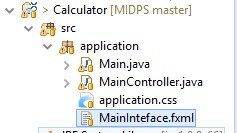
\includegraphics[scale=1.5]{a_1} \\ 
Fig a-1 - "Ierarhia structurii aplicatiei" \\
\vspace{10 mm}
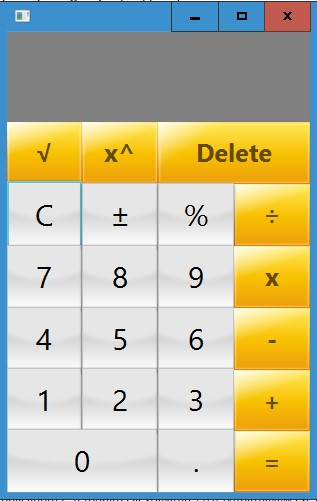
\includegraphics[scale=0.85]{a-2} \\
Fig a-2- "GUI Aplicatiei" \\
\vspace{10 mm}
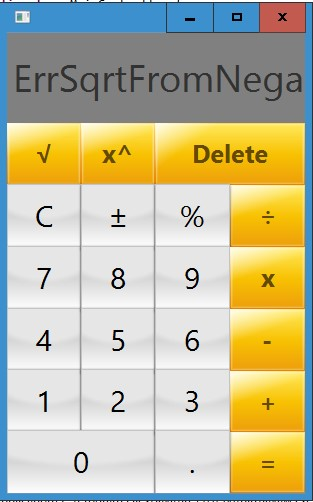
\includegraphics[scale=0.85]{b-1} \\
Fig b-1 - "Exceptia radicalului" \\
\vspace{10 mm}
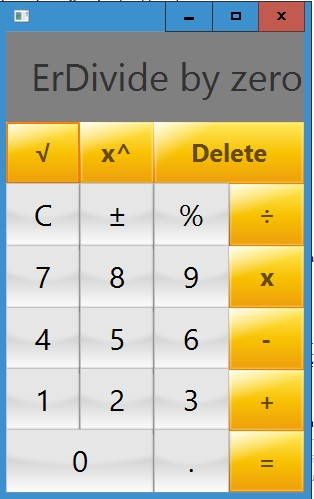
\includegraphics[scale=0.85]{b-2} \\
Fig b-2 - "Exceptia impartirii la zero" \\
\vspace{10 mm}
\lstinputlisting[style=mystyle, language=Java, caption={Main.java}, label=paymentview,]{sourcecode/Main.java}
\vspace{10 mm}
\lstinputlisting[style=mystyle, language=Java, caption={MainController.java}, label=paymentview,]{sourcecode/MainController.java}
\vspace{10 mm}
\lstinputlisting[style=mystyle, language=Java, caption={MainInterface.fxml}, label=paymentview,]{sourcecode/MainInteface.fxml}
\vspace{10 mm}
\lstinputlisting[style=mystyle, language=Java, caption={application.css}, label=paymentview,]{sourcecode/application.css}
\end{center}


